\documentclass[twocolumn]{aastex62}

\newcommand{\vdag}{(v)^\dagger}
\newcommand\aastex{AAS\TeX}
\newcommand\latex{La\TeX}
\usepackage{amsmath}
\usepackage{physics}
\usepackage{hyperref}
\usepackage{natbib}
\usepackage[T1]{fontenc}
\usepackage[english]{babel}
\usepackage[utf8]{inputenc}

\begin{document}

\title{\Large Foreløpig ingen tittel.}

\author{Håkon Tansem}

\author{Nils-Ole Stutzer}

\author{Bernhard Nornes Lotsberg}

\begin{abstract}

\end{abstract}

\section{Introduction} \label{sec:intro}
An ever occuring problem in many fields of science is a binary system of
interacting elements taking two possible values. Binary problems can be found in
everything from political science, where one could model outcomes of a vote in a
two party system, to modeling phase transitions in solid states physics. In this
paper we will focus on the latter, where we will model a time evolving
two-dimensional Ising model of interacting spins by means of a Markov Chain
Monte Carlo (MCMC) algorithm in addition to a Metropolis algorithm. We will explore how
different grid sizes and temperatures make the lattice behave, and how the systems energy and magnetization
developes in time, the final aim being to estimate the critical temperature of
the phase transition when the lattice looses its magnetization. 

This paper will present needed theory and implementation of the theory in the Method
section \ref{sec:method}, the results will be presented in the Results section
\ref{sec:results} and be discussed in the Discussion section
\ref{sec:discussion}.

\section{Method} \label{sec:method}
\subsection{The Ising Model and Important Quantities from Statistical Menchanics} \label{subsec:ising_model}
The physical system considered by this paper will be a two-dimensional Ising
model, consisting of a grid of $N\times N$ magnetic spins. Each spin can have
the value $s = +1$ ($\uparrow$) or $s = -1$ ($\downarrow$), and they interact only with their nearest neighboors. An
example of such a lattice is 
\begin{align}
	\begin{smallmatrix}
		\uparrow & \downarrow & \cdots &\uparrow \\
		\uparrow & \uparrow & \cdots & \downarrow \\
		\vdots & \ddots & \ddots & \vdots \\
		\downarrow & \uparrow & \cdots & \uparrow.
	\end{smallmatrix}
\end{align}
The energy of the lattice is defined by 
\begin{align}
	E = -J\sum_l\sum_{\langle kl\rangle} s_k s_l,
\end{align}
where $\langle kl\rangle$ denotes the sum over the nearest neighboors and the
spins take the values $s_i = \pm 1$ and $J$ has units energy. The magnetization is defined similarly as 
\begin{align}
	M = \sum_i s_i,	
\end{align} 
simply being the sum of the systems spins. The probability of the system having
a cetain energy state is given by the Boltzmann distribution 
\begin{align}
	P(E_i) = \frac{1}{Z}e^{-\beta E_i},
\end{align}

where $\beta = \frac{1}{k_B T}$ for the Boltzmann constant $k_B$ and the
temperature $T$. The partition function of the system discribing all statistical
properties of the system in equilibrium and is needed to normalize the Boltzmann
distribution is defines as the sum 
\begin{align}
	Z = \sum_i e^{-\beta E_i},
\end{align}
over all possible microstates of the system. The mean energy and absolute magnetization
of the system is then given as 
\begin{align}
	\langle E \rangle &= \sum_i E_i P(E_i) = \sum_i \frac{E_i}{Z}e^{-\beta E_i} = \pdv{\ln Z}{\beta}\\
	\langle |M| \rangle &= \sum_i |M_i| P(E_i) = \sum_i \frac{|M_i|}{Z}e^{-\beta E_i}
\end{align}
and represent the most likely state of equilibrium of the system.
Another important quantity from
thermodynamics is the heat capacity measuring the change in temperature $T$ for
a given change in the systems heat. The heat capacity at constant volume is given as 
\begin{align}
	C_V &= \dv{\langle E \rangle}{T} = \frac{1}{k_B T^2}\left(\frac{1}{Z}\sum_i E_i^2 e^{-\beta E_i} - \langle E\rangle^2\right) \\
	& = \frac{1}{k_BT^2}\left(\langle E^2\rangle - \langle E\rangle^2\right) = \frac{\sigma^2_E}{k_B T^2},
\end{align}
thus being analogous to the variance in energy states. The sum again runs over
all microstates.
Finally, the magnetic susceptibility measuring how the systems magnetization
responds to an external magnetic field, is defined as 
\begin{align}
	\chi &= \beta\left(\sum_i\frac{M_i^2}{Z}e^{-\beta E_i} - \langle |M_i|\rangle^2 \right)\\
	& = \frac{1}{k_BT}\left(\langle M^2\rangle - \langle |M|\rangle^2\right) = \frac{\sigma^2_{|M|}}{k_BT}.
\end{align} 
These thermodynamical quantities will later be usefull when estimating the
critical temperature of the phase transition when the system looses its net magnetization.

\subsection{Analytical Solutions to the $2\times2$ Lattice}\label{subsec:two_by_two_lattice}
Before discribing the algorithm modeling the time development of the lattice, we
show the analytical solutions to the mean energy and absolute magnetization as
well as the heat capacity and the susceptibility, so as to later enable a
comperison of the numerical results to known analytically quantities. When
counting the energy and magnetization of the $2\times2$ lattice as discribed in
the previous subsection we get the possible states of the system shown in Table
\ref{tab:possible_energy}. This lattice has in all $2^{N^2} = 2^4 = 16$ possible microstates. 

\begin{deluxetable}{cccc}
	%\tablewidth{0pt}
	\tablecaption{Table showing the possible energies $E_i$ and magnetizations $M_i$ of the $2\times2$ lattice and their corresponding number of spins up $N_\uparrow$ and their degenrecies $d_i$. \label{tab:possible_energy}}
	%\tablecomments{}
	\tablecolumns{4}
	\tablehead{$N_\uparrow$ & $d_i$ & $E_i$ $[J]$ & $M_i$}
	\startdata
	$4$  & $1$ & $-8$& $4$   \\
	$3$ & $4$  & $0 $& $2$\\
	$2$ & $4$  & $0 $& $0$\\
	$2$ & $2$  & $8 $& $0$\\
	$1$ & $4$ & $0 $& $-2$\\
	$1$ & $1$ & $-8$ &$-4$ 
	\enddata
\end{deluxetable}
Using the possible energy states in Table \ref{tab:possible_energy} we can write
the partition function of the system as 
\begin{align}
	Z &= \sum_i e^{\beta E_i} = e^{8J\beta} + 4 + 4 + 4 + 2e^{-8J\beta} + e^{8J\beta} \\
	&= 4\cosh(8J\beta) + 12.
\end{align}
Using this we get the expectation value for the energy to be  
\begin{align}
	\langle E\rangle  &= \frac{1}{Z}\sum_i E_i e^{-E_i\beta} \\
	&= \frac{1}{Z}\left(-8J + 2\cdot 8Je^{-8J\beta} - 8Je^{8J\beta}\right) \\
	&= -\frac{8J\sinh(8J\beta)}{\cosh(8J\beta) + 3}.
\end{align}
Similarly we find that the expectation value of the absolute magnetization is
given by 
\begin{align}
	\langle |M| \rangle &= \frac{1}{Z}\sum_i |M_i|e^{-E_i\beta} \\
	&= \frac{1}{z}\left(4e^{8J\beta} + 4\cdot 2 + 4\cdot 2 4e^{8J\beta}\right) \\
	&= \frac{2e^{8J\beta} + 4}{\cosh(8J\beta) + 3}.
\end{align}
Next this leads to the heat capacity being 
\begin{align}
	C_V &= \dv{\langle E \rangle}{T} = -\frac{1}{k_BT^2}\dv{\langle E\rangle}{\beta} \\
	&= -\frac{1}{k_BT^2}\dv{\beta}\left(-\frac{8J\sinh(8J\beta)}{\cosh(8J\beta) + 3}\right) \\
	&= \frac{192(\cosh(8J\beta) + 1)}{(\cosh(8J\beta) + 3)^2}
\end{align}

\section{Results} \label{sec:results}

\begin{figure*}
	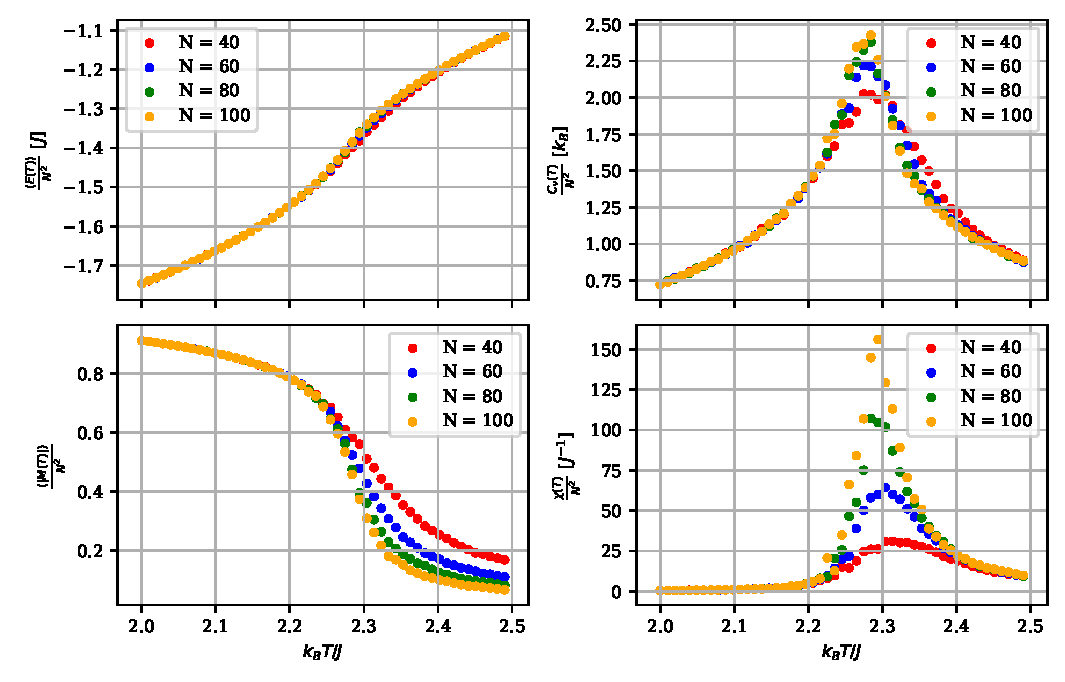
\includegraphics{{Figures/thermo_quants}.pdf}
	\caption{}
	\label{fig:thermo_quants}
\end{figure*}

\section{Discussion} \label{sec:discussion}

\section{Conclusion} \label{sec:conclusion}

\nocite{Jensen:2019}

\bibliography{ref}
\bibliographystyle{aasjournal}
\end{document}

% End of file `sample62.tex'.
